\section{Design}

\begin{figure*}[t]
	\centering
	\begin{subfigure}[t]{0.8\textwidth}
	\centering
		       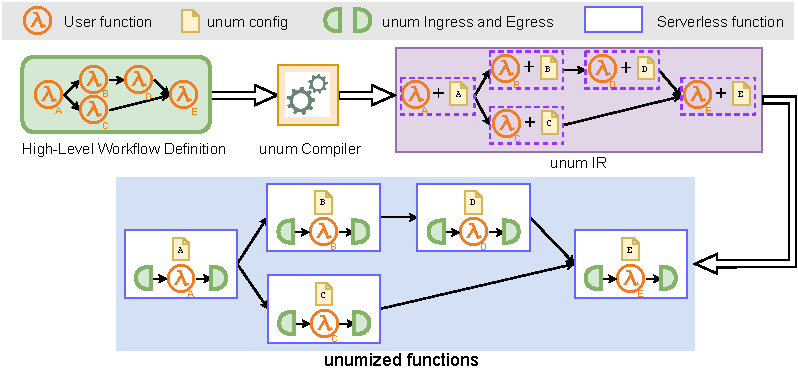
\includegraphics[width=0.8\columnwidth]{figures/unum-arch-compile-time.pdf}
		% 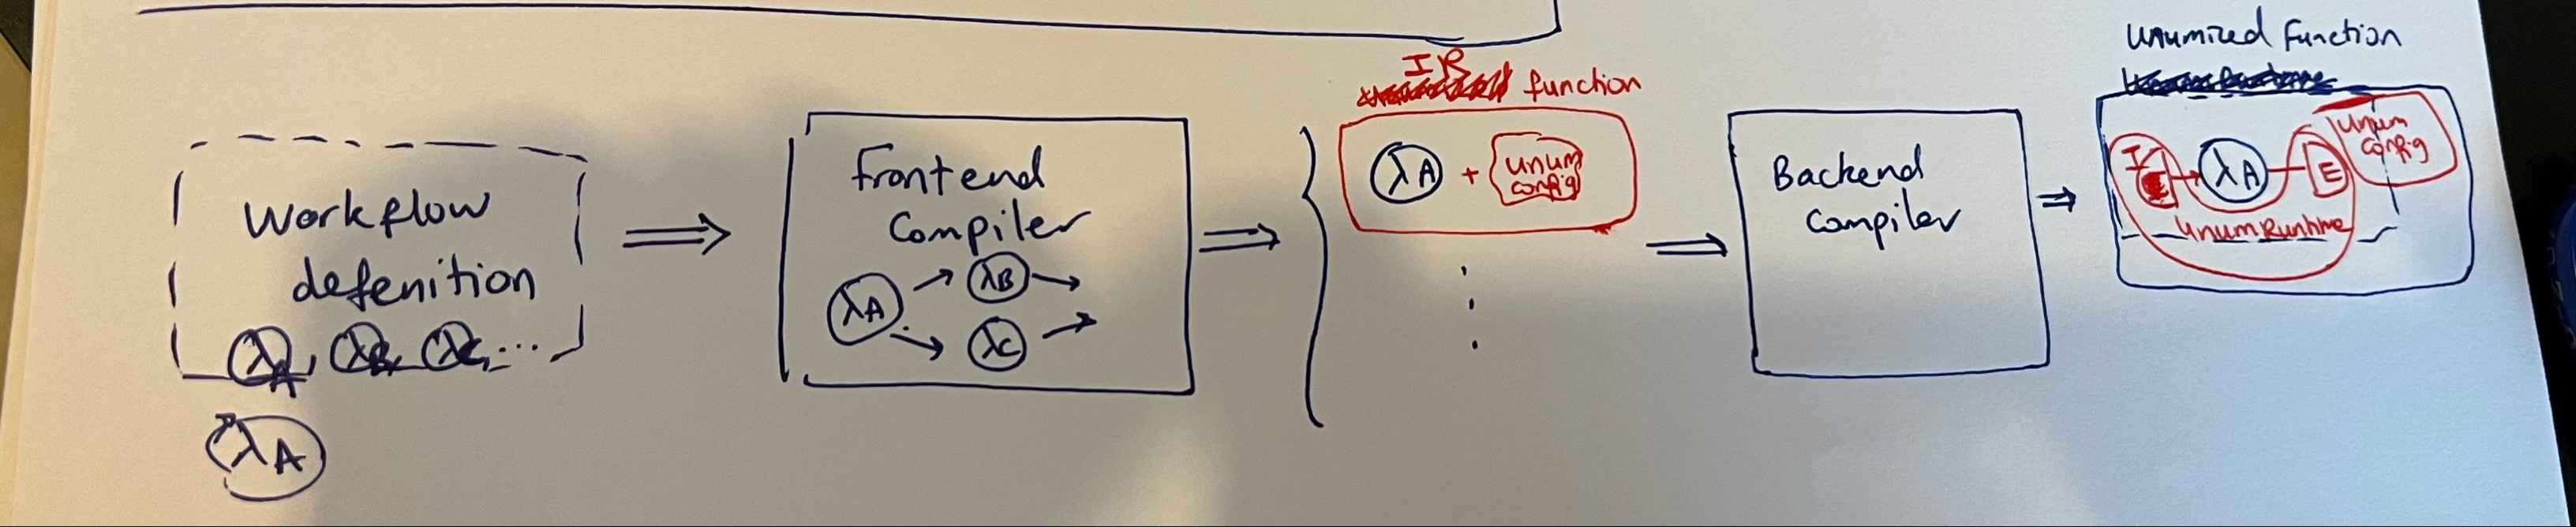
\includegraphics[width=\columnwidth]{figures/architecture.png}
		\caption{Serverless workflows form directed graphs. \name{}
		partitions the graph into an intermediate representation where each
		function is embedded with a configuration that encodes how to
		transition to its immediate downstream nodes. Developers package user
		function, \name{} config and \name{}'s runtime library (\deorc{})
		together to create unumized functions.}
		\label{fig:arch:unum-compile-time}

	\end{subfigure}
	\begin{subfigure}[b]{\columnwidth}
		\centering
		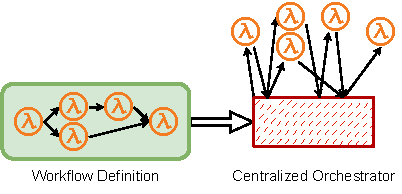
\includegraphics[width=0.8\columnwidth]{figures/unum-arch-centralized.pdf}
		\caption{A typical serverless workflow system drives workflow logic
			using a centralized orchestrator that invokes constituent
			functions and waits for their outputs.}
		\label{fig:arch:centralized}
	\end{subfigure}
	\hfill
	\begin{subfigure}[b]{\columnwidth}
		\centering
		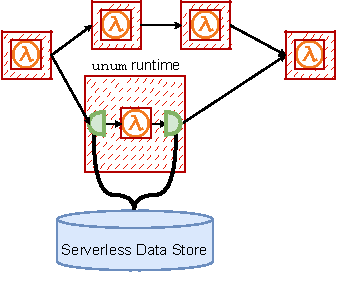
\includegraphics[width=.7\columnwidth]{figures/unum-arch-runtime.pdf}
		\caption{At runtime, \name{} orchestration logic is decentralized and
			runs in-situ with the user functions on an unmodified serverless
			platform. For synchronization and checkpointing,
			\name{} relies exclusively on a standard datastore of choice, such
			as DynamoDB or Cosmos DB.}
		\label{fig:arch:unum-runtime}
	\end{subfigure}
	\caption{\name{}'s Decentralized Orchestration. \name{} partitions
	orchestration logic at compile time and a decentralized orchestrator
	(\deorc{}) runs in-situ with user functions to perform only the
	orchestration logic local to its subsection of the graph.}
	\label{fig:arch}
\end{figure*}

To achieve the objectives in \S\ref{sec:bg}, \name{} utilizes a
design/strategy we call ``\emph{decentralized orchestration}'' where instead
of executing workflow orchestration logic entirely within a centralized
orchestrator, a set of ``decentralized orchestrators'' run \emph{in-situ} with
user functions and each performs only the orchestration logic \emph{local to
its subsection} of the workflow.

Efficiently implementing decentralized orchestration while also preserving the
benefits of centralized orchestrators (\S\ref{sec:bg:orchestrator}) requires
\name{} to solve three key challenges:

\begin{enumerate}

	\item Given a workflow written in a high-level description language, how
	to partition its orchestration logic such that it can run in a
	decentralized manner in-situ with user functions?

	\item How to efficiently execute orchestration logic in a
	decentralized manner, esp. when it requiers data sharing and
	synchronization across function instances (e.g., fan-in)?

	\item How to provide exactly-once execution semantics when the
	orchestration logic is decentralized across function instances that can
	crash and retry at any point mid-execution?

\end{enumerate}

\name{} contributes an end-to-end system that solves the three challenges and
delivers significant cost savings and improved or comparable performance than
a state-of-the-art production orchestrator (\S\ref{sec:eval}).
Figure~\ref{fig:arch} depicts
\name{}'s architecture. \shadi{the contrast part is not very clear. is it
essentially a vs b?} \dhl{Can you elaborate on \emph{why} it is not clear? a
is compile time. b and c are both runtime.}

\name{} solves the first challenge \emph{at compile time}, using a frontend
compiler and an intermediate representation (IR). Given a workflow definition
written in a high-level description language, the frontend compiler derives a
directed graph representation where nodes are user functions and edges
represent workflow transitions between functions. Based on the directed graph,
the compiler generates an IR in the form of configuration files, one file for
each node in the graph. A \name{} configuration encodes all the outgoing edges
of a node such that each function in the workflow knows how to transition just
to its immediate downstream nodes.

With the configurations from the IR, \name{} solves the second challenge using
a decentralized orchestrator (\deorc) \shadi{hard name. also, you don't have an orchestrator anymore, is this the best term? unum runtime, unum orchestrator, or unum-orch. is better in my opinion if so, at least use "deOrc" or "de-orc".} \shadi{a cosmetics point: using the texttt for so many keywords makes it hard to read. I would only use for code, function names, etc. not for unum or deorc.} that efficiently implements a set of
workflow patterns in a decentralized manner and can run in-situ with the
constituent user functions. In particular, the \deorc{} is a platform-specific
runtime library made up of an ingress component and a egress component.
Developers package each user function with its assigned \name{} configuration
and the \deorc{} to create an \emph{unumized} function. When an unumized
function executes, its entry point is no longer the user code but instead the
\deorc{} ingress. And when user code completes, it returns its results to the
\deorc{} egress which then interprets its co-located \name{} configuration and
performs the workflow transition.

A critical complexity is to enable fan-in patterns where a single ``sink''
function aggregates the results of multiple upstream functions. Importantly,
to avoid idle-billing (\S\ref{sec:bg}), we want the entire fan-in pattern to
execute \emph{wait-free}, i.e., to invoke the sink function only when all its
input upstream functions have completed. To this end, \name{} leverages a
shared \emph{intermediary data store} that is a strongly consistent \shadi{why? no motivation given} serverless
storage (e.g., DynamoDB) with conditional store operations \shadi{why? no motivation given}. Upstream functions
each writes user code output into and synchronizes over the intermediary data
store such that faster functions simply terminate and only the last-to-finish
function invokes the sink function. \shadi{I would not talk about fan-in here. you have not mentioned why we need fan-in, it comes out of the blue.}

\name{} leverages again the intermediary data store to also solve the third
challenge and provide \emph{exactly-once} execution semantics. \name{} uses
checkpointing, where each function checkpoints its output to the intermediary
data store, to limit the scope of retries when workflows crash mid-execution
and guarantee that even if there are multiple instances of the same function,
concurrent or not, only one instance's output is taken as the final result and
propargates downstream. \shadi{do we need to describe this here? if you move fan-in the data store is a bit out of the blue. it can work, but you can also just give fwd pointer in the 3 challenges at the beginning of the section.}

In the rest of the section, we first describe how the \name{} IR encodes
transitions between functions (\S\ref{sec:ir}), then explains how \deorc{}
efficiently executes transitions in a decentralized manner, and finally we
detail \name{}'s checkpointing mechanism and how it ensure exactly-once
execution semantics. \shadi{do we want to have Ir first or second?}

\subsection{\name{} Intermediate Representation}\label{sec:ir}

\begin{figure*}[t!]
	\centering
	\begin{subfigure}[t]{\columnwidth}
		\centering
		\begin{minted}[
			frame=single,
			fontsize=\scriptsize
			]{json}
{
	"Name": "F",
	"Next": {
		"Name": "G",
		"InputType": "Scalar",
		"Conditional": true,
	}
}
		\end{minted}
		\caption{\texttt{chain} pattern that invokes function \texttt{G} with
			\texttt{F}'s result}
		\label{fig:gadget-examples-chain}
	\end{subfigure}
	\begin{subfigure}[t]{\columnwidth}
		\centering
		\begin{minted}[
			frame=single,
			fontsize=\scriptsize
			]{json}
{
	"Name": "M",
	"Next": {
		"Name": "N",
		"InputType": "Map"
	}
}
		\end{minted}
		\caption{\texttt{map} pattern that invokes a parallel instance of
			\texttt{N} for each element of the vector output of \texttt{M}}
		\label{fig:gadget-examples-map}
	\end{subfigure}
	\hfill
	\begin{subfigure}[t]{\columnwidth}
		\centering
		\begin{minted}[
			frame=single,
			fontsize=\scriptsize
			]{json}
{
	"Name": "G",
	"Next": [
	{
		"Name": "H",
		"InputType": "Scalar"
	},
	{
		"Name": "M",
		"InputType": "Scalar"
	}
	]
}
		\end{minted}
		\caption{\texttt{fan-out} pattern that invokes function \texttt{H} and
			\texttt{M} with the result of \texttt{G}}
		\label{fig:gadget-examples-fanout}
	\end{subfigure}
	\begin{subfigure}[t]{\columnwidth}
		\centering
		\begin{minted}[
			frame=single,
			fontsize=\scriptsize
			]{json}
{
	"Name": "N",
	"Next": {
		"Name": "S",
		"InputType": {
			"Fan-in": {
				"Values": [
				"N-unumIndex-*"
				]
			}
		}
	}
}
		\end{minted}
		\caption{\texttt{fan-in} pattern that invokes function \texttt{S} with
			the result of all \texttt{N} instances of a \texttt{map}.}
		\label{fig:gadget-examples-fanin}
	\end{subfigure}

	\begin{subfigure}[t]{\columnwidth}
		\centering
		\begin{minted}[
			frame=single,
			fontsize=\scriptsize
			]{json}
{
	"Name": "F",
	"Next": [
	{
		"Name": "G",
		"InputType": "Scalar",
		"Conditional": "$ret < 0"
	},
	{
		"Name": "H",
		"InputType": "Scalar",
		"Conditional": "$ret >= 0"
	}
	]
}
		\end{minted}
		\caption{\texttt{F} branches on the user function's result by
		combining \texttt{fan-out} with \texttt{Conditional}}
		\label{fig:gadget-examples-branch}
	\end{subfigure}

	\begin{subfigure}[t]{\columnwidth}
		\centering
		\begin{minted}[
			frame=single,
			fontsize=\scriptsize
			]{json}
{
    "Name": "F",
    "Next": {
        "Name": "F",
        "InputType": {
            "Fan-in": {
                "Values": [
                    "F-unumIndex-$0",
                    "G-unumIndex-($0+1)"
                ]
            }
        },
        "Conditional": "$0 < $size-1"
    },
    "Next Payload Modifiers": ["$0=$0+1"]
}
		\end{minted}
		\caption{\texttt{fold} pattern that folds \texttt{F} on the output of
		a vector of \texttt{G} functions}
		\label{fig:gadget-examples-fold}
	\end{subfigure}

	\caption{The \name{} IR representation of common transition patterns.}
	\label{fig:ir-examples}
\end{figure*}
\shadi{the paper suddenly jumps into details of the IR. we still haven't established how we are doing the decentralized orchestration, which is much more important than the IR syntax. I would first discuss the deorc, how the patterns are supported and then the IR.} \shadi{I like the high-level architecture, but this section forward has too much details too soon. We should have a discussion on the flow of this and the next section.}

Before executing serverless workflows in a decentralized manner, a workflow
definition first needs to be partitioned such that each function performs only
the orchestration logic local to its subsection of the workflow. The \name{}
intermediate representation solves this problem with a naming scheme that
uniquely identifies each function instance in the workflow and a configuration
language in JSON that encodes workflow transitions.\shadi{this is another instance of jumping to details without the big picture. you suddenly talk about naming structure and json without giving the details of what this config contains (the following sentences)} Specifically, each
function is assigned a configuration that contains: i. \textit{which}
function(s) to run next, ii. \textit{when} the next function(s) should run,
iii. \textit{what} input should the next function(s) run with.

Note that the IR configuration is platform-agnostic. In particular, it does
not specify how to launch the next function(s), and how to send input data to
the next function(s). These details are left to the \name{} runtime library
(\deorc{}) that can target specific platforms (for example, the \deorc{} for
AWS runs functions as lambdas and uses the Lambda asychronous invocation API
to launch functions). Thus, workflows are portable across platforms by simply
changing the \deorc{} library.

The \name{} frontend compiler can generate IR from workflow definitions
written in high-level description languages (e.g., AWS Step Functions), but
developers can also write IR configurations directly, with just a few lines of
JSON. In particular, The \name{} IR uses a top-level \texttt{Name} field to
identify the source function that the configuration is co-located with, a
\texttt{Next} field to list the workflow transitions, and under which a
\texttt{Name}, \texttt{Conditional}, and \texttt{InputType} fields that
identify which function to run, when and with what input.
Figure~\ref{fig:ir-examples} shows examples on how to express common
orchestration patterns such as branching, chaining, map, fan-out, fan-in and
fold: 

\dhl{Sync with background. should have at least mentioned some of those patterns in
the background.}

\shadi{you suddenly jump into these patterns. why these? where did they come from? this might be the right place to have the apps discussed.}

\paragraph{chain}

%Chaining is a simple but common orchestration pattern. For example, an
%application might include a function (the source) that processes input data
%from a sensor followed by another function (the target) that adjusts an
%actuator based on the processed input. The \texttt{chain} pattern connects the
%two functions by invoking the target function with the source function's
%result.

Figure~\ref{fig:gadget-examples-chain} expresses a chain with a \texttt{Next}
field that contains a single JSON object whose \texttt{InputType} is
\texttt{Scalar}. \texttt{Scalar} means that the target function (i.e.,
\texttt{G}) should receive as input the source function's (i.e., \texttt{F}'s)
output as a singular entity. The \texttt{Conditional: true} means that this
transition should always take place whenever \texttt{F} produces a result.
\texttt{Conditional} is assumed to be \texttt{true} when not specified.

\paragraph{fan-out}

%Another common pattern processes the output of a function in different ways in
%parallel. For example, an social network application might perform several
%independent functions given a new user post, such as URL shortening and
%resolving other users mentioned in the post. The \texttt{fan-out} pattern
%launches a vector of functions (branches) each with the output of the same
%source function.

Figure~\ref{fig:gadget-examples-fanout} expresses a fan-out with an array in
the \texttt{Next} field. Each item of the array identifies a different target
function that should should run in parallel. The \texttt{InputType} field is
\texttt{Scalar} for both branches because both should receive as input the
source function's (i.e., \texttt{F}'s) output as a singular entity.

\paragraph{map}

%An application may also perform the same function on multiple outputs of a
%source function. For example, a photo management application might unpack an
%archive of high-resolution images in one function and perform compression on
%each of the resulting images. The \texttt{map} pattern invokes the same
%function once for each element in a vector of outputs from the source
%function.

Figure~\ref{fig:gadget-examples-map} expresses a \texttt{map} with a
\texttt{Next} field that contains a single JSON object whose
\texttt{InputType} is \texttt{Map}, which indicates that the source function's
(i.e., \texttt{F}'s) output should be treated as an array and for each
element, a target function (i.e., \texttt{G}) should launch with that element
as the input.

\paragraph{fan-in}

%After processing data with many parallel branches, applications commonly want
%to aggregate results. For example, a video encoder might divide a large video
%into chunks, encode each in parallel and then concatenant all the encoded
%chunks together. The \texttt{fan-in} pattern invokes a single ``sink''
%function with the outputs from a vector of functions (the fan-in branches).

Figure~\ref{fig:gadget-examples-fanin} expresses a \texttt{fan-in} with a
\texttt{Next} field that contains a single JSON object whose
\texttt{InputType} is \texttt{Fan-in} under which a \texttt{Values} fields
specifies an ordered list with names of functions whose results should be the
target function's (i.e., \texttt{S}'s)input.

Different from \texttt{Scalar} and \texttt{Map} where the target function only
depends on the source function's output, \texttt{Fan-in} expresses data
dependencies across functions which is difficult to implement efficiently. We
discuss how we support \texttt{fan-in} in \S\ref{sec:runtime}.

\paragraph{branch}

%An application may decide to take a different branch of the workflow graph
%based on runtime behavior (e.g., the output of a function). The
%\texttt{branch} pattern selects a next function based on some boolean
%condition.

Figure~\ref{fig:gadget-examples-branch} expresses a \texttt{branch} with an
array in the \texttt{Next} field where each branch has a \texttt{Conditional}.
Notice that \texttt{branch} is expressed similarly as \texttt{fan-out}
combined with the \texttt{Conditional} field. This example demonstrates the
flexibility and expressiveness of \name{} IR's building blocks which
developers can compose to express additional patterns.

\paragraph{fold}

In functional programming, \texttt{fold} is higher-level function that takes
another functions and applies it to an vector of values. In serverless
workflow, \texttt{fold} is an advanced pattern that is supported by few
systems~\cite{azure-functions}. Although \name{} is built on a simpler
abstraction without adding new components, we support folding a function on
the output of a vector of functions.

Figure~\ref{fig:gadget-examples-fold} expresses a \texttt{fold} that folds the
function \texttt{F} on a vector of \texttt{G} instances result, using a
combination of \texttt{Fan-in}, \texttt{Conditional} and \texttt{Next Payload
Modifiers}. On a high-level, \texttt{F} recursively calls itself, passing the
previous iteration's output (\texttt{F-unumIndex-\$0}) and the next \texttt{G}
instance's result (\texttt{F-unumIndex-(\$0+1)}), until it reaches the last
\texttt{G} instance in the vector ((\texttt{Conditional: "\$0<\$size-1"})). On
each iteration, \texttt{F} increments its index by 1 (\texttt{"\$0=\$0+1"}).
We explain the details on \name{} IR's naming scheme and the use of index and
runtime variables (e.g., \texttt{\$0}) in the next section.


\subsubsection{Naming and Dynamic Runtime Behavior}\label{sec:ir:naming}

A key design challenge of the \name{} IR is to support dynamic runtime
behavior with statically generated configurations.

For instance, in a workflow that consists of a \texttt{map} followed by a
\texttt{fan-in}, \texttt{map} creates multiple parallel instances of the same
function, but the number of instances depends on the output data and cannot be
known at compile-time. \name{} needs to uniquely identify each function
instance so that \texttt{fan-in} can execute correctly (e.g., not miss an
instance or counting the same instance twice).

To solve this problem, \name{} defines a naming scheme for runtime instances
and exposes a set of APIs to interact with names. First,
\name{} requires each user function to have a user-defined name (in the
top-level \texttt{Name} field). This is also a common requirement for existing
serverless systems when developers deploy their functions. Next, each branch
in a \texttt{map} and \texttt{fan-out} pattern is assigned an integer index,
starting from zero, and the $i^th$ branch is named
\texttt{<FunctionName>-unumIndex-\emph{i}}. For nested fan-outs, the indexes
are delimited with periods. For example,
\texttt{<FunctionName>-unumIndex-\emph{i.j}} identifies the $i^{th}$ branch in
the outer loop and $j^{th}$ in the inner loop.

To identify all branches, the \name{}~IR supports glob patterns, such as
\texttt{*}, when specifying runtime instances' names.
Figure~\ref{fig:gadget-examples-fanin} shows a \texttt{fan-in} example that
invokes \texttt{S} with the outputs from all instances of \texttt{N}.

\name{} IR provides a set of runtime variables and APIs that enables
additional dynamic behavior. For example, \texttt{\$0} refers to the
inner-most index of the function instance which can be used in the
\texttt{Values} field for fan-in when input depends on specific instances
instead of all instances. The \texttt{Next Payload Modifiers} field allows
expressions that can modify the runtime variables (e.g., \texttt{\$0=\$0+1}),
which can implement fold or for loops when combined with a termination
condition in \texttt{Conditional}.


\name{} IR also provides other APIs that interacts with runtime data, such as
\texttt{\$ret} that refers to the function's output, and \texttt{\$size} that
refers to the number of parallel branches in a \texttt{map}.




\subsection{Decentralized Orchestration with \deorc{}}\label{sec:runtime}

\begin{figure}[t!]
	\centering
	\scalebox{1}{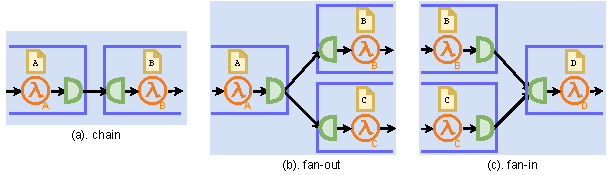
\includegraphics[width=\columnwidth]{figures/deorc-patterns.pdf}}
	\caption{\deorc{} implements transitions in a decentralized manner where
the egress on the source function(s) and ingress on the target function(s)
work together to execute the orchestration. \shadi{does this figure add value given you have Fig 1. you can probably combine the patterns there ans name them there and reuse that figure.}}
	\label{fig:transition}
\end{figure}

\begin{figure}[]
    \begin{minted}[
    frame=single,
    fontsize=\scriptsize
  ]{json}
{
    "Data": {
        "Source": "http | dynamodb | s3 | ...",
        "Value": "<object> | [<pointers>]"
    },
    "Session": "uuid",
    "Fan-out": {
        "Index": "int",
        "Size": "int",
        "OuterLoop": {
            "Index": "int",
            "Size": "int"
        }
    }
}
    \end{minted}
    \caption{\name{} runtime input payload schema}
    \label{fig:input-format}
\end{figure}

The second challenge of \name{} is to efficiently implement decentralized
orchestration. \name{} designs a decentralized orchestrator (\deorc) that
consists of an ingress and an egress component and can run in-situ with
constituent user functions. \deorc{} transparently interposes on user code
entry and exit so that it does not change how developers write application
code.

The primary purpose of \deorc{} is to interpret IR configurations and implement
transitions with platform-specific APIs. In particular, \deorc{} implements
transitions in a decentralized manner where the egress on the source
function(s) and ingress on the target function(s) work together to execute the
transition.

A key requirement of \deorc's design is to only use the basic serverless
abstraction without relying on any specialized APIs. Therefore, we designed
\deorc{} such that it only depends on two serverless components that are
universally supported by all platforms: i. a FaaS system that supports
asynchronous invocation of functions (e.g., AWS Lambda, Azure Functions,
Google Cloud Funtions, Openwhisk) and ii. a strongly consistent data store
that supports conditional write operations (e.g., DynamoDB, Cosmos DB).

Figure~\ref{fig:transition} depicts how \deorc{} executes \texttt{chain},
\texttt{map} and \texttt{fan-in}. The other patterns described in
\S\ref{sec:ir} are variations of these three patterns.

\paragraph{chain} 

The \texttt{chain} pattern involves one egress on source function and one
ingress on the target function. When the \texttt{Next} field of the source
function's \name{} config contains a single object whose \texttt{InputType} is
\texttt{Scalar}, the \deorc{} egress simply invokes the target function with
the source function's user code's output. \deorc{} uses asynchronous
invocation to avoid waiting and idle-billing and a particular input payload
schema in JSON (Figure~\ref{fig:input-format}) that contains \name{} runtime
metadata.

When the target function is invoked, the input is first received by the \deorc{}
ingress. The ingress uses the \texttt{Data} field to read the user function's
input data. If the \texttt{Source} is \texttt{http}, the input data is
directly embedded in the \texttt{Value} field. Otherwise,
\name{} uses the pointers in \texttt{Value} to read the input data from the
intermediary data store. Finally, ingress calls its user function and passes
it the input.

\paragraph{fan-out}

The \texttt{fan-out} pattern involves one egress on the source function and
many ingresses on the target functions.

Similar to chaining, the egress asynchronously invoke each target and the
ingresses on targets read the input data sent from the source and passes it to
its user function.

\texttt{map} is a simple variation of \texttt{fan-out} where the egress treats
its user code output as an iterable. \texttt{branch} is another variation
where the egress first evaluates the boolean condition in \texttt{Conditional}
before invoke the target function in that branch.

\paragraph{fan-in}

The \texttt{fan-in} pattern involves one ingress node and many egress nodes.
It is the main complexity of decentralized orchestration as we want to ensure
that the transition is \emph{wait-free} to avoid idle-billing. In particular,
we want to invoke the sink function only when all upstream functions have
completed so that the sink function does have to be spun up ahead of time and
wait for upstream functions to finish. Moreover, the upstream functions should
simply terminates when done instead of waiting for each other either.

To achieve this, the \deorc{} egress always writes the output of its user
function to a data store when its \name{} config has a \texttt{InputType} of
\texttt{Fan-in}. This serves two purposes: (1). it allows any of the upstream
functions to access the output of other upstream functions (2). it signals the
completion of a function. This way, each egress can simply writes its output
and terminate. Other egress nodes can still access completed egress' data
after they terminate. Any one of the egress can invoke the sink function. And
any one of the egress can see if other egress has completed or not.

Strongly consistent data store is important because it prevents the
scenarios where all egress have written outputs but none of them sees that all
have completed, which results in the sink function never invoked.

Additionally, \texttt{fan-in} makes sure that when the sink function is
invoked, it is invoked only once. \name{} achieves this by having the egress
nodes synchronize with each other via the same data store such that only the
last-to-finish egress invokes the sink function. Synchronization is done with
atomic read-after-write over a single object. Specific implementation depends
on the data store and we discuss the details in \S\ref{sec:impl}.

The last-to-finish egress invokes the sink function with a vector of pointers
to each upstream function's stored output. The pointers are the in same order
as the vector of upstream function names. The ingress on the sink function
dereferences each point by reading from the data store and passes a vector of
output values to its user function.


\subsubsection{Runtime Metadata}

To support a rich variety of orchestration patterns, \name{} requires a
specific input payload schema in JSON (Figure~\ref{fig:input-format}) that
contains \name{} runtime metadata. In particular, \name{} uses the
\texttt{Fan-out} field to store branch indexes. The \texttt{Fan-out} field
contains a recursive \texttt{OuterLoop} field that \name{} uses to support
nest fan-outs. The \texttt{\$0} and \texttt{\$size} variable in
\name{} IR (\S\ref{sec:ir}) refers to the \texttt{Index}  and \texttt{Size}
field of the top-level \texttt{Fan-out} field.

The runtime additionally uses a \texttt{Session} field to support concurrent
invocations of the same workflow. The \texttt{Session} field is a UUID string
that is unique to a workflow invocation and shared by all constituent function
instances in the invocation. Function checkpoint names
(\S\ref{sec:exec-gntee}) are prefixed by the \texttt{Session} string so that
concurrently invocations do not overwrite each other's data. We discuss
\name{} checkpoints and execution guarantees details in the next section.


\subsection{Execution Guarantees}\label{sec:exec-gntee}

An important characteristic of any workflow system is (a) how it deals with  a
transient failure in a constituent step, and (b) what guarantees it makes in
the presence of such faults.
 
Many workflow systems durably persist progress to limit the scope of re-execution after faults
\cite{aws-step-functions, durable-functions, netherite, google-workflows, kappa}.
In \name{}, each function is checkpointed to storage after it
completes. In particular, if a workflow experiences crashes mid-execution,
\name{} does not retry from the beginning but from the node of failure only.

\name{} guarantees \textbf{exactly-once execution}, meaning that each step of
the workflow appears to execute exactly once. FaaS engines already
support automatic retries for functions; however, they only guarantee at-least-once
execution. Strengthening this guarantee requires dealing with the following
subtleties:

\begin{itemize}
	\item Function executions are not always deterministic, each re-execution
	may produce a different result.
	\item Some FaaS engines may detect failures incorrectly, thus multiple
	executions of a function can be in progress simultaneously.
\end{itemize}

Fortunately, we found a way to handle these challenges by taking advantage of
conditional store operations supported by strongly consistent data stores.
Specifically, \name{} guarantees that even if there are multiple function
execution instances, concurrent or not, only one instance's result is taken as
the final result and propagates to the downstream ingress node(s). Other
instances simply discard their results and terminate.

\paragraph{Checkpoints and Synchronization.}%\name{} uses a similar checkpointing technique across all transition patterns. 
After user code completes, the \name{} egress gadget immediately writes a checkpoint file that contains the user code
results to the intermediary data store. The checkpoint is uniquely named with
the instance's name (i.e., the name according the
\name{}~IR's naming scheme (\S\ref{sec:ir:naming}), prefixed by the workflow
invocation's unique session ID) such that the existence of a checkpoint
implies the corresponding function has successfully completed its user
function. The create operation is a conditional write and only succeeds when
the file does not already exist. If there are concurrent duplicate instances,
only one of them will create the checkpoint. The others will receive an error
from the write operation and \name{} runtime will simply terminate the
instance. The instance that successfully creates a checkpoint will proceeds to
executing its egress node and propagate its result to downstream functions.

For nonconcurrent duplicates (e.g., retries), \name{} checks if a checkpoint
exists \emph{before} running its user code. If a checkpoint does not exist,
\name{} goes ahead and runs the user code. Otherwise, \name{} reads the data
from the checkpoint and use that as final result without running user code
again. Then \name{} will run the ingress node to invoke the downstream function.
This is necessary because the duplicate might be a retry whose prior execution
crashed after checkpointing but before running the downstream ingress node. \name{} can
tolerate running a ingress/egress node more than once because of the same protection
against duplicates.

\paragraph{External Side Effects.} In the applications targeted by \name{},
there is no need for functions to directly call external storage services.
Rather, all functions are "side-effect-free": their only effect is to provide
a result. 

%Therefore, the "exactly-one-result" guarantee of the \name{} runtime
%is in fact synonymous with exactly-once execution.

Although it is not currently required by any of our applications, it is
conceivable to extend \name{} in the future to support exactly-once execution even for workflows whose
functions have additional side effects. For example, a store interposition
mechanism (such as used in Beldi \cite{beldi}) could be added to support
functions that require more complex storage interactions than obtaining an
input and producing a result.